% Full instructions available at:
% https://github.com/elauksap/focus-beamertheme

\documentclass{beamer}
\usetheme{focus}

\title{Enzymbasierte digitale Biosensoren f{\"u}r medizinische Anwendungen}
%\subtitle{Biosensoren in Kombination mit Biocomputing}
\author{Maren Krafft}
%\titlegraphic{
\includegraphics[scale=1.25]{focuslogo.pdf}}
\institute{Universit{\"A}t Passau \\ Lehrstuhl f{\"u}r technische Informatik}
\date{02 08 2018}

\AtBeginSubsection[]
{
	\begin{frame}<beamer>{Gliederung}
	\tableofcontents[currentsection,currentsubsection]
	\end{frame}
}
\begin{document}
    \begin{frame}
        \maketitle
    \end{frame}

	\begin{frame}{Motivation}
		\begin{itemize}
			\item Mehrere Inputs k{\"o}nnen direkt verarbeitet werden
			\item Bietet neue M{\"o}glichkeiten im medizinischen Bereich
			\item Beispiele: 
			\begin{itemize}
				\item nicht nur einzelne Substanzen analysieren, sondern krankheitsabh{\"a}ngige Kombinationen von chemischen Substanzen
				\item feedback loops
				\item personalisierte Medikation
				\item zeitnahe Reaktion
			\end{itemize}
		\end{itemize}
	\end{frame}
   
    \begin{frame}{Outline}
    \tableofcontents
    % You might wish to add the option [pausesections]
	\end{frame}

	\section{Begriffserkl{\"a}rung}
	\begin{frame}{Wichtige Begriffe}
		\begin{itemize}
			\item Enzyme =
			\item biochemische Substanzen =\\
			\item Biosensoren = 
		\end{itemize}		
	\end{frame}
 
 	\section{Konzept}
 	
 	\subsubsection{Biosensoren}
 	
 	\begin{frame}<beamer>{Gliederung}
 	\tableofcontents[currentsection,currentsubsection]
 	\end{frame}
 	
    \begin{frame}{Biosensoren}
       Aufbau: 
        \begin{figure}[H] \centering 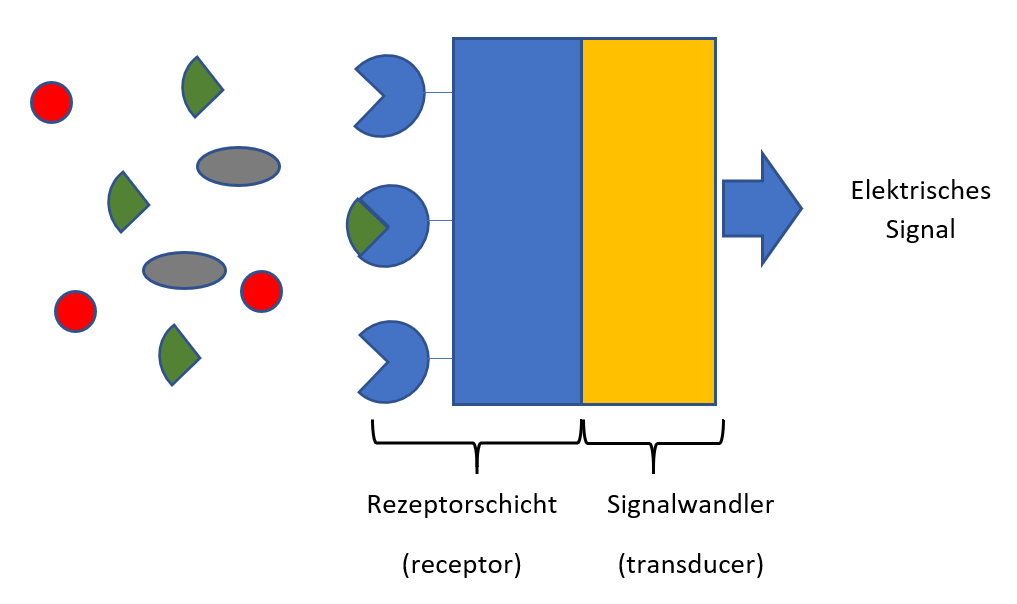
\includegraphics[scale= 0.33]{pics/biosensor.png} \caption{Eigene Darstellung} \label{img:and} 	
       \end{figure}
    \end{frame}



	\subsubsection{Enzymbasierte Logikgatter}
	
	\begin{frame}<beamer>{Gliederung}
	\tableofcontents[currentsection,currentsubsection]
	\end{frame}

    \begin{frame}{Enzymbasierte Logikgatter}
    Umsetzung uns bekannter Logikgatter durch biochemische Substanzen
    
    	\begin{itemize}	
    		\item Enzyme als Logik
    		\item 2 biochem. Substanzen als Input
    		\item Reaktion mit dem Enzym produziert eine andere biochemische Substanz
    		\item Vorhandensein eines bestimmten biochem. Stoffes als Booleanwerte 1 und 0
    	\end{itemize}     
    \end{frame}
        
    \begin{frame}{Enzymbasierte Logikgatter - Beispiel 'AND'}
    
    Enzyme: Gox = Glucose-Oxidase und Cat = Katalase\\
    Inputs: Glucose und H\textsubscript{2}O\textsubscript{2}
    
     \begin{figure}[H] \centering 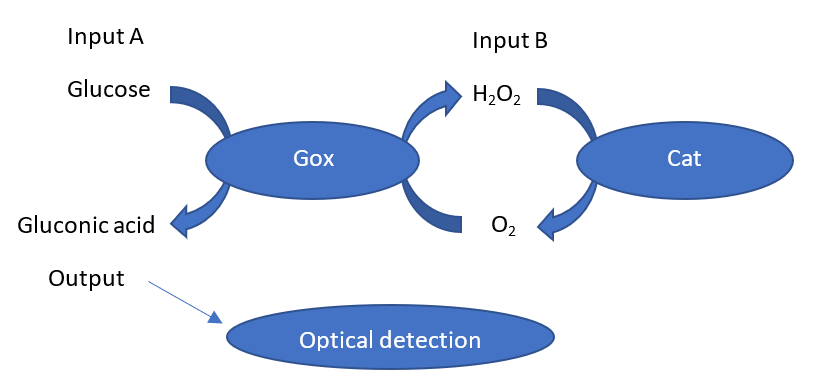
\includegraphics[scale= 0.33]{pics/ANDneu.png} \caption{Eigene Darstellung nach \cite{hallo4} } \label{img:and} 	
   	 \end{figure}
  
    \end{frame}


    \subsubsection{enzymbasierte Biosensoren}
    
    \begin{frame}<beamer>{Gliederung}
    \tableofcontents[currentsection,currentsubsection]
	\end{frame}
    
    \begin{frame}{Netzwerke aus enzymbasierten Logikgattern}
    	Durch Kombination mehrerer enzymbasierter Logikgatter ist es m{\"o}glich ein Netzwerk zu erschaffen.
    	
    	Beispiel: 
    	\begin{itemize}
    		\item Enzyme: ADH(Alkoholhydrogenase), GDH(Glucose-Dehydrogenase), GOX(Glucose-Hydrogenase)
    	\end{itemize}
    	\begin{figure}
    		\centering \scriptsize 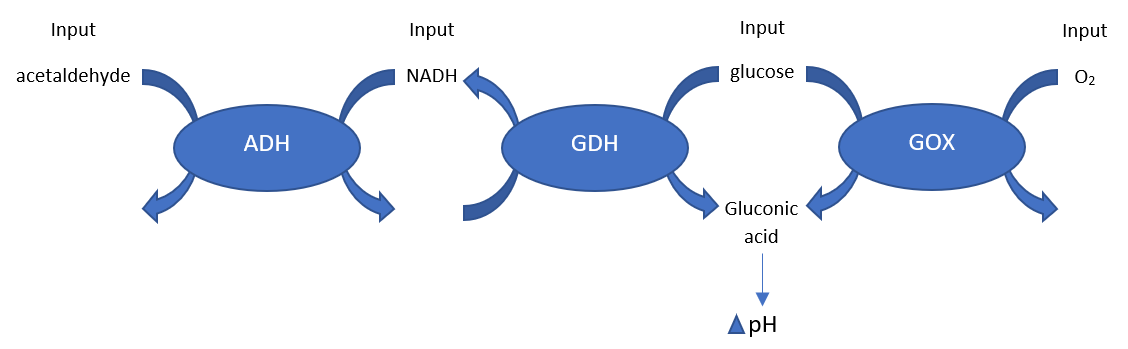
\includegraphics[scale= 0.30]{pics/network1.png}
    	\caption{Network, composed of enzyme-based logic gates} 
   		\end{figure}
   		
   	
    
	\end{frame}

	\begin{frame}{Netzwerke aus enzymbasierten Logikgattern}
	
	\begin{figure}
		\centering \scriptsize 
		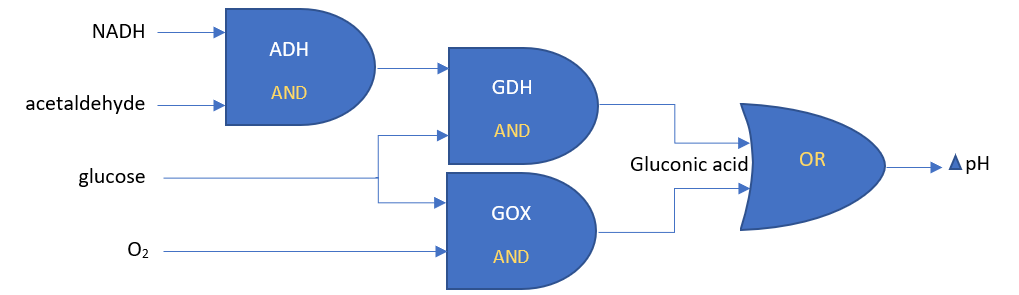
\includegraphics[scale = 0.30]{pics/network2.png} \caption{Darstellung nach \cite{hallo4}} 
	\end{figure}

	\begin{figure}[H] \centering \includegraphics[scale= 0.20]{pics/pH.png} \caption{Inputs/Voltage} \label{img:ph} 
	\end{figure}
	\end{frame}


	\begin{frame}{Kombination mit einem Signalwandler}
	
		Durch Hinzufügen eines Signalwandlers zu einem Netzwerk bestehend aus enzymbasierten Logikgattern ist es möglich einen Biosensor zu erschaffen, der mehrere Inputs erhält und verarbeiten kann.\\
		Anhand des Beispiels:\\
        \begin{figure}[H] \centering \includegraphics[scale= 0.37]{pics/pH.png} \caption{Inputs/Voltage} \label{img:ph} 
        \end{figure}
        
    \end{frame}
    
   \section{F{\"u}r medizinische Anwendungen}
   
   \begin{frame}{Design f{\"u}r medizinische Analyseanwendungen}
  	Um
  
   \begin{table}
   	\scriptsize
   	\begin{tabular}{l|c|c|c|c|c|}
   	condition & norepiquinone & NADH & glucose & lactate & norepinephrine\\ \hline
   	traumatic brain injury & 1&0&0&1&1\\
   	hemorrhagic shock & 1&1 &1&1&1\\
   \end{tabular}\\
   \end{table}


   
	\end{frame}

   

   \section{{\"U}berlegungen}
   
   

	\appendix
	\begin{frame}[allowframebreaks]{Quellen}
	\nocite{*}
	\bibliography{demo_bibliography}
	\bibliographystyle{plain}

	\end{frame}
    
    
\begin{frame}[focus]
Vielen Dank f{\"u} Ihre Aufmerksamkeit
\end{frame}
   
\end{document}
